
\documentclass[sigplan,screen,9pt]{acmart}
\settopmatter{printfolios=true,printccs=false,printacmref=false}

%%
%% \BibTeX command to typeset BibTeX logo in the docs
\AtBeginDocument{%
  \providecommand\BibTeX{{%
    \normalfont B\kern-0.5em{\scshape i\kern-0.25em b}\kern0.8em\TeX}}}

\setcopyright{none}

\usepackage{alltt}
\usepackage{svg}

\title{Synthetic Datasets Mimicking Real World Completions}
\author{Milan W. M. Binz}
\date{September 2022}

\begin{document}

\maketitle

\section{Motivation}
Today most studies on Code Completion use synthetic datasets, such as Py150K, to train and evaluate their models.
Such datasets are created by mining large amounts of code from Github, or other code repositories; They are not specifically created for code completion models but for other adjacent Code related tasks.
In training, random tokens in the code are selected, then all the code following the selected tokens is hidden from the model. The model is tasked with either predicting the next token or a sequence of subsequent tokens.
This is done due to the assumption that these datasets are good analogs for the completions required by real programmers.
Findings from Hellendoorn et. al.\cite{8812116}, which were corroborated by Aye et. al.\cite{https://doi.org/10.48550/arxiv.2011.04542}, show that this assumption does not hold.
Both found a significant drop in accuracy when testing models trained on synthetic datasets on datasets consisting of completions real developers had used. 
See Figure \ref{fig:accuracies}.

Aye et. al.\cite{https://doi.org/10.48550/arxiv.2011.04542} additionally found that a model trained on real world performance outperforms a model trained on synthetic data. 
Furthermore Aye et. al.\cite{https://doi.org/10.48550/arxiv.2011.04542} also documented that developers use tools developed with synthetic datasets less often than those trained on real world data.


\begin{figure}
    \centering
    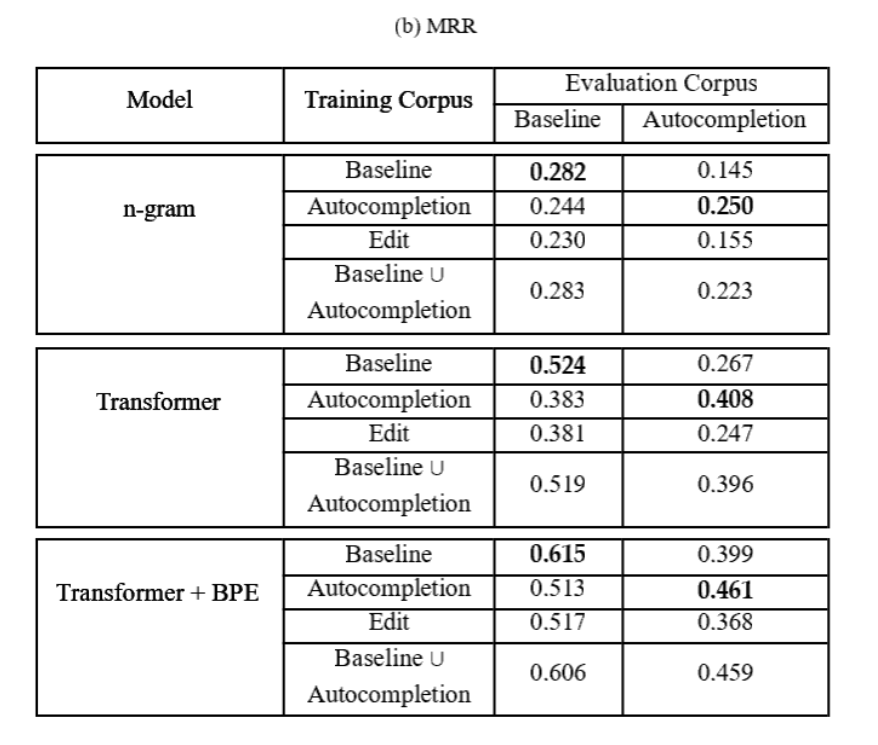
\includegraphics[scale = 0.33]{accuracies.png}
    \caption{Accuracies as reported by Aye et. al.
    \cite{https://doi.org/10.48550/arxiv.2011.04542}}
    \label{fig:accuracies}
\end{figure}

This begs the question, why researchers continue to use these synthetic datasets, instead of real world data?
One possible reason might be the lack of large publicly available datasets of real world completions.
While the dataset used by Hellendoorn et. al.\cite{8812116} was made public, it is sourced from only 86 developers.
Due to its small size, its usefulness as a training set is very low, meaning that its mostly only useful as a verification set.
The much larger dataset used by Aye et. al.\cite{https://doi.org/10.48550/arxiv.2011.04542}, which contains more than three million completions collected from Facebook developers over a time span of several months, was not made public.

This shows the difficulties involved with creating a large corpus of real world completions.
To create such a dataset one first needs access to hundreds if not thousands of programmers over a long time. When a company collects the completions, the likelihood that these completions contain code not meant to be publicly available, or industry secrets, is quite high, which would make publication of such a dataset impossible.

If one considers the fact that some tools such as github copilot were created with much larger datasets than many other current models\cite{2107.03374}, we see that, in order to create a dataset large enough to be used by such a model, one would need even more programmers and more time to observe their completions, making the creation of such a dataset not a viable approach.

While the creation of a larger publicly available dataset of real world completions is desirable, instead I propose the creation of an synthetic dataset more simmiliar to real world data.
This means that the access to so many programmers is no longer required. Once an approach to create such a dataset has been shown to be effective, this would make the creation of other comparable datasets easier, allowing for more programming languages to be covered, and for creating larger datasets as needed while still minimizing concept drift.


\section{Adapting an already existing dataset}
%Aye et. al.\cite{https://doi.org/10.48550/arxiv.2011.04542} explored how big the impact of differences between code which is still in production and code which has been finished, gone through qualitiy control and been published hypothesizing that these differences might account for some of the concept-drift.
%The fact that they did not find noticeable performance differences points to the selection of completion instances being the main difference maker.
%Starting from an already existing dataset of raw code the objective is to select which tokens the model should predict.
%Instead of just selecting tokens randomly, I propose selecting them in a way that matches the distribution of token types observed in real world completions, as documented by Hellendoorn et. al.\cite{8812116} and Aye et. al.\cite{https://doi.org/10.48550/arxiv.2011.04542}.  See Figure \ref{fig:distributions}.

%Additionally, instead of just controlling for token types it may be useful to also account for the length of the tokens, in order to prevent the created dataset being "easier" than real world data and to further minimize concept drift. This should select tokens which are more similar to the tokens programmers actually ask to be completed.


%This means one could use a publicly available dataset such as Py150k as a starting point and instead of selecting completion instances randomly control the selection more closely.
%I propose to select the completion instances in such a way that the distribution of various token types, such as method invocations, variables, etc, matches the distributions reported by aye et. al.\cite{https://doi.org/10.48550/arxiv.2011.04542} and hellendoorn et. al\cite{8812116} as closely as possible.


%The efficacy of such a dataset can then be shown by using the dataset of Hellendoorn et. al. as a validation set and comparing the accuracy of a model trained on the dataset used as a starting point and a model trained on the created dataset.

Of the differences Hellendoorn et al. documented between Completion Instances randomly chosen from synthetic data sets and those real programmers require three appear interesting and could be accounted for in the selection process:
\begin{enumerate}
    \item {\bf Token type distribution}
     Real code completions favor Method-Invocations to a much larger degree than artificial ones additionally Variable and Class names are significantly over-represented in artificial completions both appearing more than twice as much as they do in real completions(see Figure \ref{fig:distributions})
    \item {\bf Token Length}
    Artificial completions are with an average length of 9.06 characters noticeably shorter than real ones which are on average 9.87 characters long
    \item {\bf Token Placement}
    In their paper proposing the CodeFill model Izadi et. al. \cite{Izadi_2022} also proposed their approach to improve artificial completions Cardinal Point Prediction.
    Their approach works by restricting Completions to only occur after specific Tokens such as dots or opening brackets this approach can also be included in this work to study both how effective it is on its own and to explore its impact when combined with the approach outlined here.
    Izadi et al. did not test their approach against real world data.    
\end{enumerate}



\section{evaluation}
Once the datasets are created and some models have been trained both on them and on a baseline dataset the C\# versions can be evaluated against the dataset provided by Hellendoorn et al.\cite{8812116} by using that dataset as an evaluation dataset.
If the created datasets work as theorized the models trained on them should perform significantly better than the baseline models.
Another possibility is to ask Aye et al. whether they would be willing and capable to assist in the evaluation step and run the same procedure as described before on their dataset creating results for the python versions as well without them having to release their data.


%\section{Related Works}
%{\bf When Code Completion Fails: a Case Study on Real-World Completions}
%This paper by Hellendoorn et. al.\cite{8812116} was the first to showcase the loss of accuracy when evaluating models trained on synthetic datasets on real world Completions.
%To do so they collected a dataset consisting of almost 200,000 completion events from 66 developer. Only 24\% of the suggestions were accepted by programmers


%{\bf Learning Autocompletion from Real-World Datasets}


%{\bf CodeFill}
%In their paper proposing their CodeFill model Izadi et. al. \cite{Izadi_2022} tried a simmiliar approach to 

\begin{figure}
    \centering
    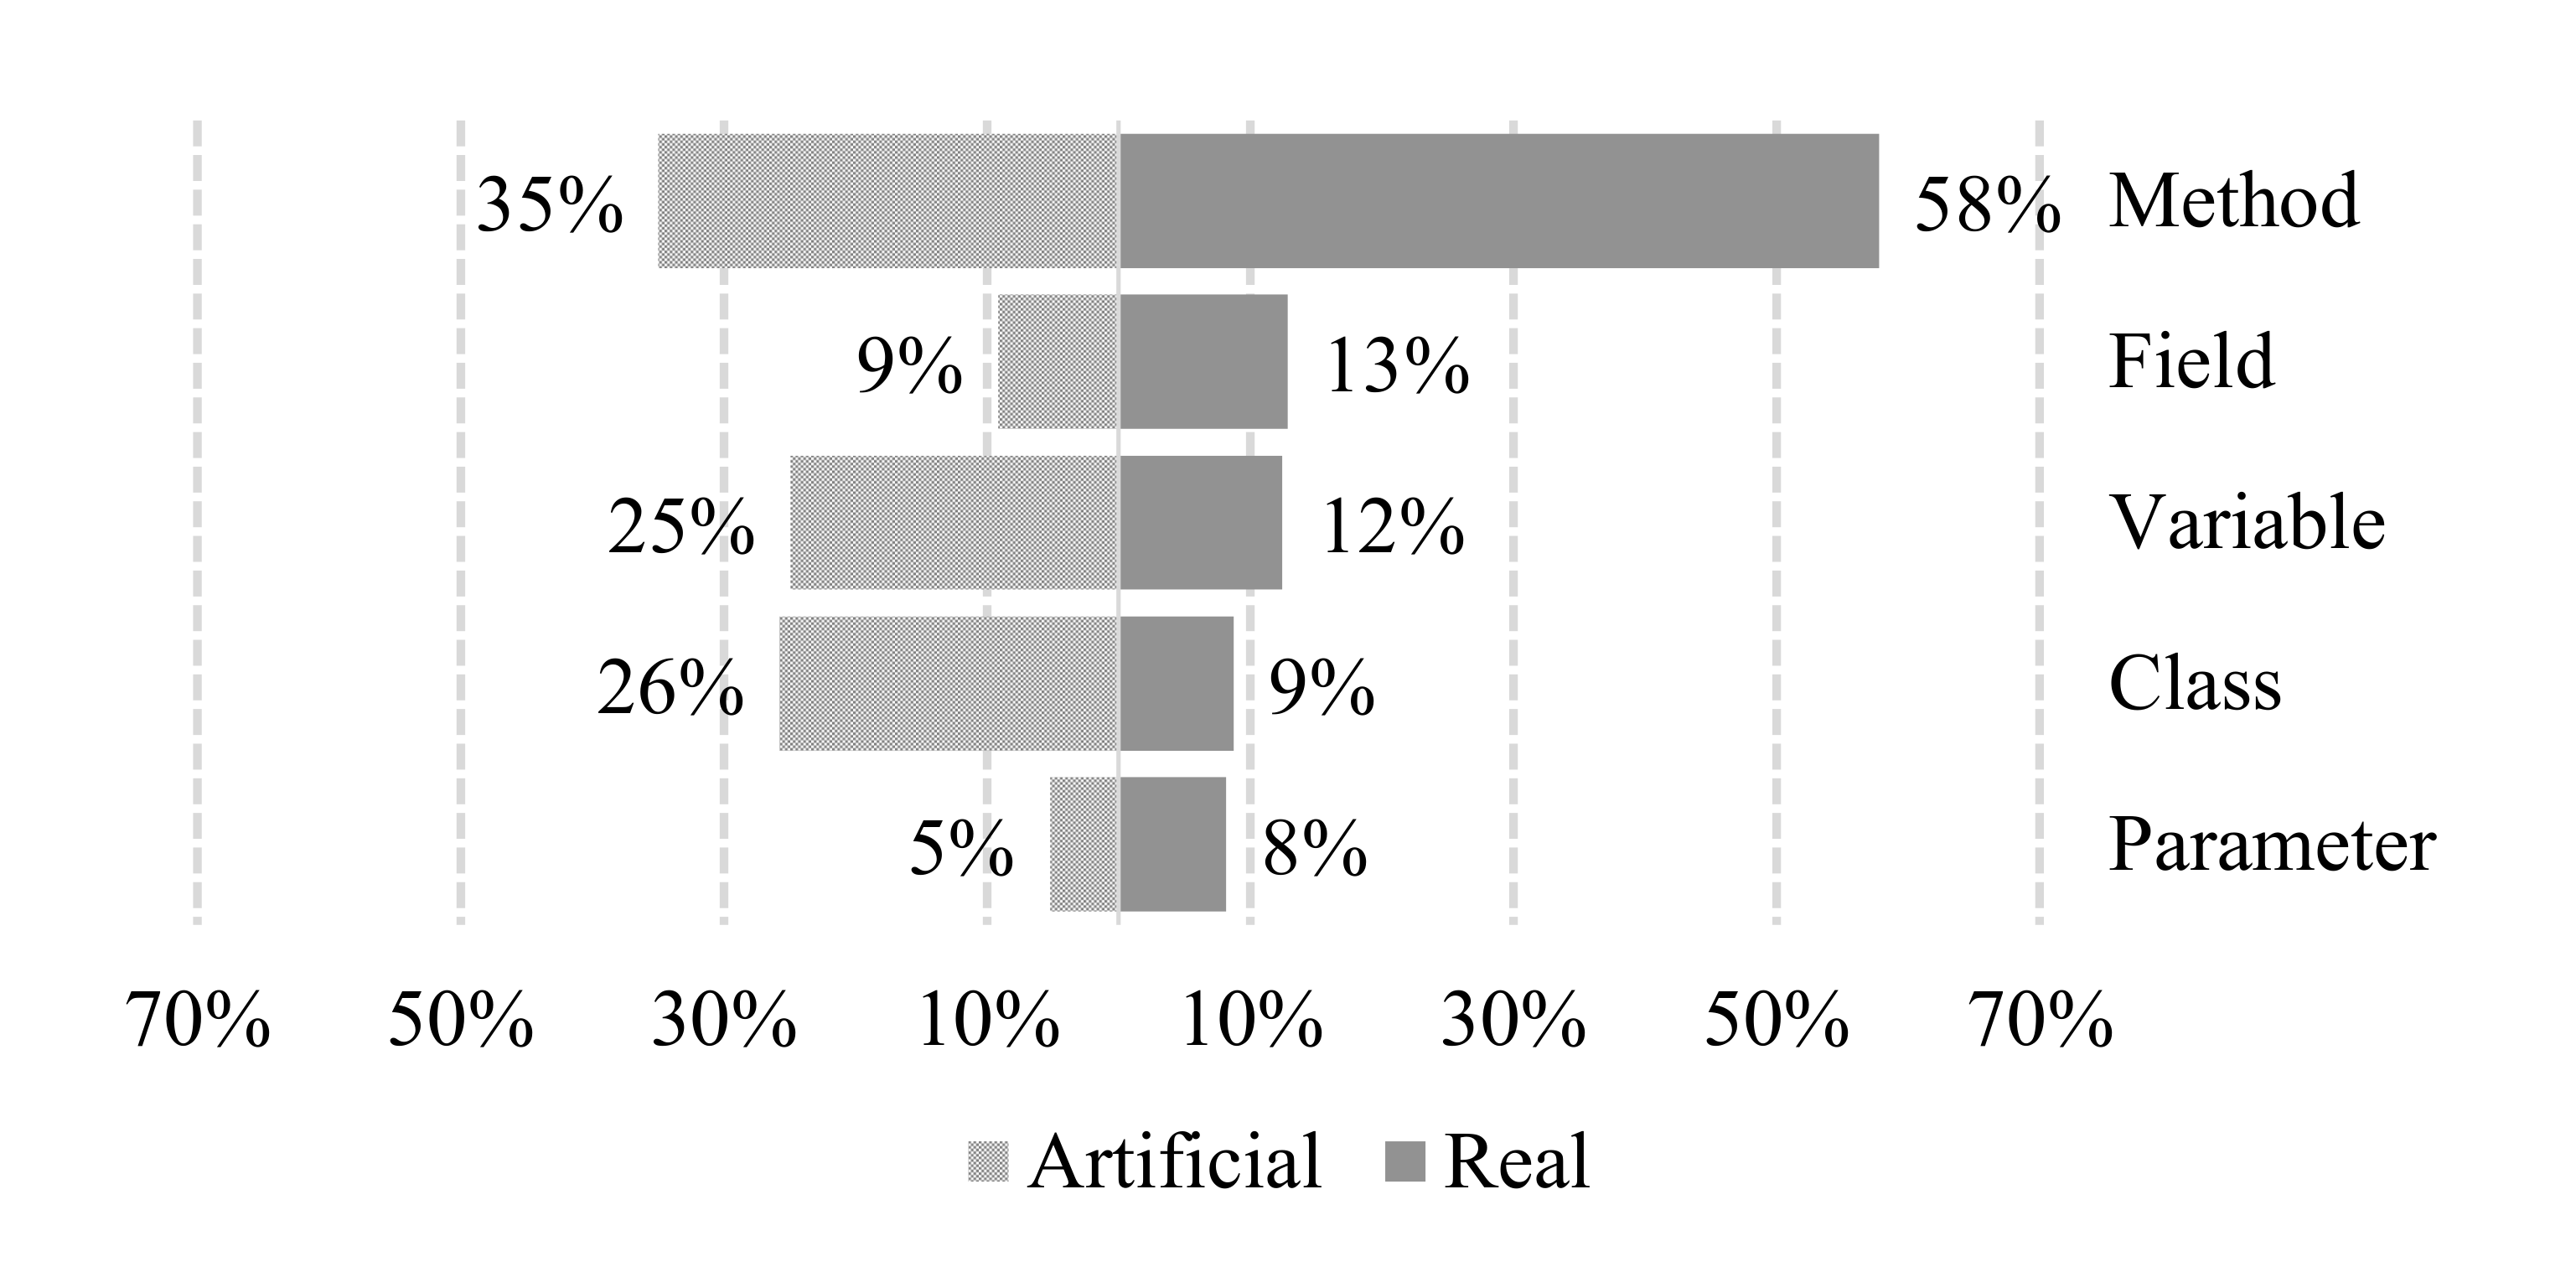
\includegraphics[scale = 0.1]{token-distribution.png}
    \caption{token distributions as reported by Hellendoorn et. al.\cite{8812116}}
    \label{fig:distributions}
\end{figure}





%References
\bibliographystyle{ACM-Reference-Format}
\bibliography{references}

\end{document}
